\documentclass[11pt,a4paper]{article}
\usepackage[a4paper,margin=1in]{geometry}
\usepackage{graphicx}
\usepackage{float}
\usepackage{booktabs}
\usepackage{hyperref}
\usepackage{amsmath}
\usepackage{listings}
\usepackage{xcolor}
\lstset{
    basicstyle=\ttfamily\small,
    breaklines=true,
    breakatwhitespace=false,
    frame=single,
    numbers=left,
    numberstyle=\tiny,
    showstringspaces=false,
    columns=fullflexible,
    keepspaces=true,
    captionpos=b
}
\usepackage{tikz}
\usetikzlibrary{positioning, arrows.meta}
\usepackage{caption}
\usepackage{subcaption}
\setlength{\intextsep}{12pt plus 4pt minus 4pt}
\setlength{\textfloatsep}{14pt plus 6pt minus 6pt}
\setlength{\floatsep}{14pt plus 6pt minus 6pt}
\hypersetup{colorlinks=true,linkcolor=blue,urlcolor=blue,citecolor=blue}
\title{Streamlit Expense Analytics: Visualization-Driven Personal Finance Dashboard}
\author{Liv Grewal (1424000076) \and Gurman (1424000041)}
\date{December 2025}

\begin{document}
\maketitle

\begin{abstract}
This report presents a web-based expense analytics platform built with Streamlit, SQLite, and Plotly. The system delivers full expense CRUD, budgeting, savings goals, alerting, and reusable visualizations. Recent enhancements add quicker expense entry, stable multi-row editing with session persistence, richer dashboard controls, and inline rendering of saved PNG plots.
\end{abstract}

\section{Introduction}
Personal finance tools often lack transparent analytics and reusable visual evidence for reports. This project provides a lightweight yet expressive dashboard that unifies data collection, analysis, and visualization with minimal setup.

\section{Problem Statement}
Users need a frictionless way to capture daily expenses, monitor budgets, and visualize spending trends without complex installations. The system must persist data, provide alerts near budget thresholds, and export visuals for documentation.

\section{Objectives}
\begin{itemize}
  \item Deliver CRUD operations for expenses with categories and payment methods, plus fast-add presets.
  \item Provide monthly and custom-range analytics with interactive charts and inline saved PNGs.
  \item Support budgeting, savings goals, and configurable spending alerts (default 80\%), with slider+input sync.
  \item Auto-save plots (pie, daily trend, monthly comparison) for academic and managerial reporting.
\end{itemize}

\section{Literature Review}
Lightweight dashboards using Streamlit have proven effective for rapid prototyping of analytics tools. SQLite remains a dependable embedded database for single-user desktop or small team scenarios. Plotly offers interactive exploration, while Matplotlib generates publication-ready images.

\section{System Architecture}
The architecture follows a layered pattern separating UI, services, and persistence. Streamlit orchestrates user interactions; service classes encapsulate analytics and budgeting logic; SQLite ensures durable storage. Figure~\ref{fig:architecture} highlights the data paths; saved plots flow to the `plots/` directory for inline viewing in Analytics.

\begin{figure}[H]
  \centering
  \resizebox{\textwidth}{!}{
  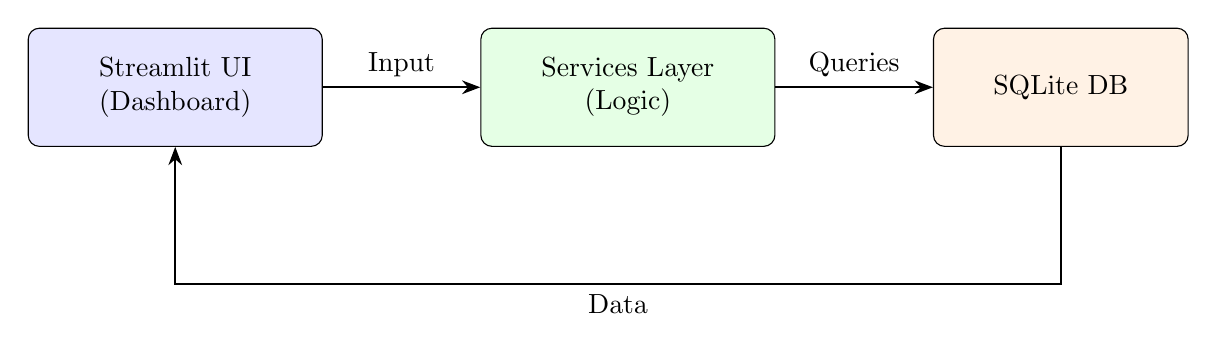
\begin{tikzpicture}[node distance=1.5cm and 2cm, >=Stealth, auto,
      block/.style={draw, rounded corners, fill=blue!10, text width=3.5cm, align=center, minimum height=1.5cm},
      service/.style={draw, rounded corners, fill=green!10, text width=3.5cm, align=center, minimum height=1.5cm},
      db/.style={draw, rounded corners, fill=orange!10, text width=3cm, align=center, minimum height=1.5cm}]
    
    \node[block] (ui) {Streamlit UI\\(Dashboard)};
    \node[service, right=of ui] (services) {Services Layer\\(Logic)};
    \node[db, right=of services] (db) {SQLite DB};
    
    \draw[->, thick] (ui) -- node[above] {Input} (services);
    \draw[->, thick] (services) -- node[above] {Queries} (db);
    \draw[->, thick] (db) |- ++(0,-2.5) -| node[pos=0.25, below] {Data} (ui);
  \end{tikzpicture}
  }
  \caption{High-level system architecture.}
  \label{fig:architecture}
\end{figure}
\vspace{8pt}

\section{Database Design}
The database uses three tables shown in Table~\ref{tab:schema}. A single SQLite file (`expenses.db`) resides in the `data/` directory for portability.

\begin{table}[H]
  \centering
  \begin{tabular}{p{3cm}p{3cm}p{7cm}}
    \toprule
    Table & Key Fields & Purpose \\
    \midrule
    expenses & id (PK), date, amount, category, payment\_method, notes & Stores atomic expense records. \\
    budgets & id (PK), month (unique), budget, savings\_goal, created\_at & Tracks monthly budgets and goals. \\
    settings & key (PK), value & Persists alert thresholds and preferences. \\
    \bottomrule
  \end{tabular}
  \caption{SQLite schema overview.}
  \label{tab:schema}
\end{table}

\section{Data Flow Diagrams}
Figure~\ref{fig:dfd0} illustrates Level 0 with user interaction points; Figure~\ref{fig:dfd1} expands analytics and budgeting paths.

\begin{figure}[H]
  \centering
  \resizebox{0.9\textwidth}{!}{
  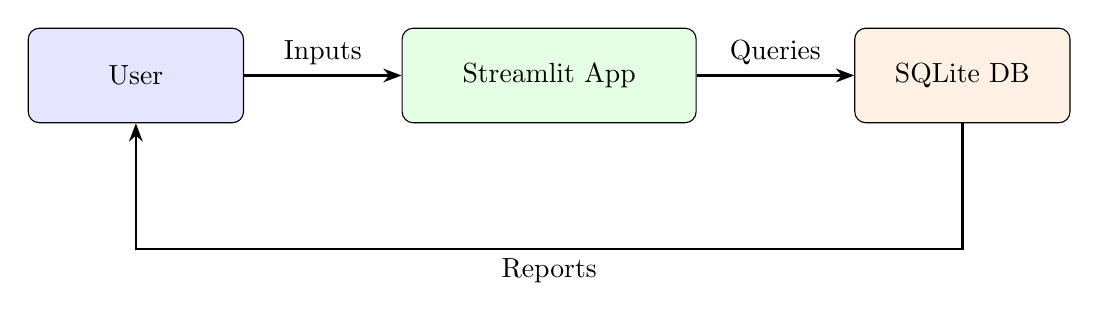
\begin{tikzpicture}[node distance=1.5cm and 2cm, >=Stealth, auto,
      user/.style={draw, rounded corners, fill=blue!10, text width=2.5cm, align=center, minimum height=1.2cm},
      app/.style={draw, rounded corners, fill=green!10, text width=3.5cm, align=center, minimum height=1.2cm},
      db/.style={draw, rounded corners, fill=orange!10, text width=2.5cm, align=center, minimum height=1.2cm}]
      
    \node[user] (user) {User};
    \node[app, right=of user] (process) {Streamlit App};
    \node[db, right=of process] (store) {SQLite DB};
    
    \draw[->, thick] (user) -- node[above] {Inputs} (process);
    \draw[->, thick] (process) -- node[above] {Queries} (store);
    \draw[->, thick] (store) |- ++(0,-2.2) -| node[pos=0.25, below] {Reports} (user);
  \end{tikzpicture}
  }
  \caption{DFD Level 0: User-system-data interaction.}
  \label{fig:dfd0}
\end{figure}
\vspace{8pt}

\begin{figure}[H]
  \centering
  \resizebox{\textwidth}{!}{
  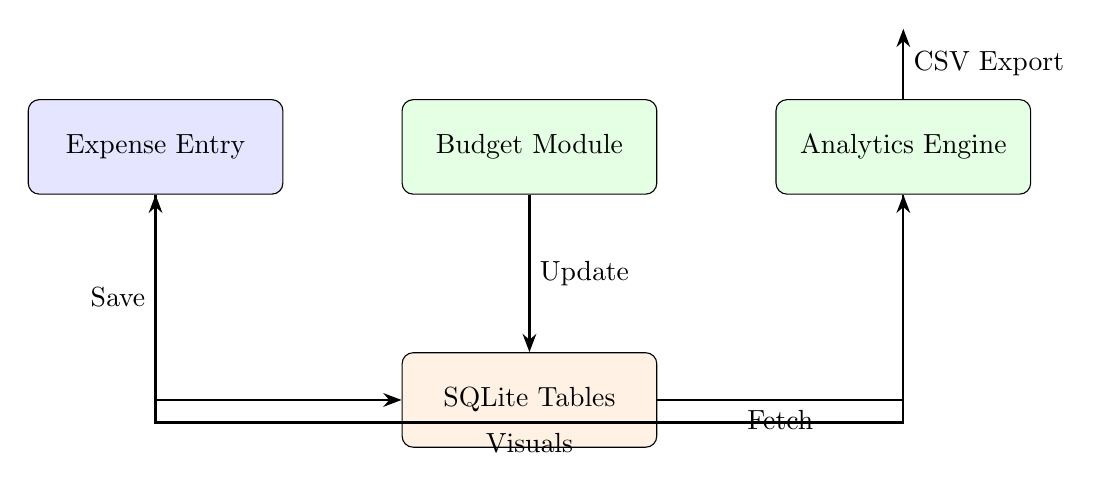
\begin{tikzpicture}[node distance=2cm and 1.5cm, >=Stealth, auto,
      comp/.style={draw, rounded corners, align=center, minimum height=1.2cm, text width=3cm}]
      
    \node[comp, fill=blue!10] (entry) {Expense Entry};
    \node[comp, fill=green!10, right=of entry] (budget) {Budget Module};
    \node[comp, fill=green!10, right=of budget] (analytics) {Analytics Engine};
    \node[comp, fill=orange!10, below=of budget] (store) {SQLite Tables};
    
    \draw[->, thick] (entry) |- node[near start, left] {Save} (store);
    \draw[->, thick] (budget) -- node[right] {Update} (store);
    \draw[->, thick] (store) -| node[near start, below] {Fetch} (analytics);
    
    \draw[->, thick] (analytics) -- ++(0,1.5) node[midway, right] {CSV Export};
    \draw[->, thick] (analytics) -- ++(0,-3.5) -| node[pos=0.25, below] {Visuals} (entry);
  \end{tikzpicture}
  }
  \caption{DFD Level 1: Expense, budget, and analytics flows.}
  \label{fig:dfd1}
\end{figure}
\vspace{8pt}

\section{Implementation Details}
The UI is organized into sidebar navigation tabs. Expenses use a two-column form with quick-amount presets and prefilled defaults; management occurs through a selectable data grid with multi-delete and multi-row edit capabilities. Analytics queries leverage Pandas for aggregation, optimized with Streamlit caching (`@st.cache_data`) for performance. Matplotlib saves PNGs for the report while Plotly powers interactive charts. Budgets and alerts are persisted in SQLite, with synchronized slider and numeric inputs.

\section{Streamlit Application Walkthrough}
The application is divided into focused sections accessible from the sidebar, each designed for a specific phase of the personal finance workflow.

\subsection{Dashboard}
The Dashboard serves as the command center, providing immediate visibility into financial health. It features:
\begin{itemize}
    \item \textbf{Key Metrics}: Real-time display of Total Spent, Monthly Budget, and Remaining Budget.
    \item \textbf{Interactive Charts}: Users can toggle between different time ranges (Current Month, Last 30 Days, YTD) and view breakdowns by Category or Payment Method.
    \item \textbf{Trend Analysis}: A line chart visualizes spending velocity over time.
\end{itemize}
Figure~\ref{fig:ui} shows the dashboard interface with these metrics and charts active.

\begin{figure}[H]
  \centering
  \includegraphics[width=0.9\textwidth]{../screenshots/streamlit_dashboard.png}
  \caption{Streamlit dashboard with metrics and charts.}
  \label{fig:ui}
\end{figure}

\subsection{Add Expense}
The "Add Expense" module is optimized for speed. It defaults to the current date and remembers the last used category and payment method to reduce friction. A "Save \& Add Another" feature allows for rapid batch entry of receipts without reloading the page.

\begin{figure}[H]
  \centering
  \includegraphics[width=0.8\textwidth]{../screenshots/add_expense.png}
  \caption{Add Expense interface with presets.}
  \label{fig:add_expense}
\end{figure}

\subsection{Manage Expenses}
This section provides a powerful data grid interface. Users can:
\begin{itemize}
    \item Filter expenses by date range, category, or text search.
    \item Select multiple rows via checkboxes.
    \item Click "Edit selected" to open a session-persistent bulk-edit table. IDs are locked to ensure integrity, while other fields remain modifiable. 
    \item Perform bulk deletions or batch updates in a single transaction.
\end{itemize}

\begin{figure}[H]
  \centering
  \includegraphics[width=0.9\textwidth]{../screenshots/manage_expenses.png}
  \caption{Manage Expenses grid with multi-select.}
  \label{fig:manage}
\end{figure}

\subsection{Analytics}
The Analytics engine drives deeper insights. It generates three key visualizations that are automatically saved as static assets for reporting:
\begin{itemize}
    \item \textbf{Category Distribution}: A pie chart (Figure~\ref{fig:cat}) revealing the largest spending areas.
    \item \textbf{Daily Trend}: A time-series plot (Figure~\ref{fig:trend}) to identify spending spikes.
    \item \textbf{Monthly Comparison}: A bar chart (Figure~\ref{fig:monthly}) comparing spending across months.
\end{itemize}

\begin{figure}[H]
  \centering
  \includegraphics[width=0.7\textwidth]{../plots/category_distribution.png}
  \caption{Category distribution pie chart.}
  \label{fig:cat}
\end{figure}

\begin{figure}[H]
  \centering
  \includegraphics[width=0.75\textwidth]{../plots/daily_trend.png}
  \caption{Daily spending trend.}
  \label{fig:trend}
\end{figure}

\begin{figure}[H]
  \centering
  \includegraphics[width=0.78\textwidth]{../plots/monthly_comparison.png}
  \caption{Decluttered month-wise spend.}
  \label{fig:monthly}
\end{figure}

\subsection{Budgets \& Goals}
Users can set a monthly budget and a savings goal. The interface uses a synchronized slider and number input, ensuring both ease of adjustment and precise value entry. Visual progress bars indicate how close the user is to their limit.

\begin{figure}[H]
  \centering
  \includegraphics[width=0.8\textwidth]{../screenshots/budgets.png}
  \caption{Budget configuration with synced sliders.}
  \label{fig:budgets}
\end{figure}

\section{Algorithms Used}
Core computations involve grouping by category for pie-chart proportions, daily aggregation for line trends, and period-based grouping for month-wise bars. Budget alerts evaluate the ratio $r = \tfrac{spent}{budget}$ and trigger when $r \ge 0.8$ by default.

\section{Code Snippets}
\begin{lstlisting}[language=Python, caption=Backend Service: Adding an expense to SQLite]
@staticmethod
def add_expense(data: Dict[str, Any]) -> int:
    return execute(
        "INSERT INTO expenses(date, amount, category, payment_method, notes) VALUES (?, ?, ?, ?, ?)",
        (
            data["date"],
            float(data["amount"]),
            data["category"],
            data["payment_method"],
            data.get("notes", ""),
        ),
    )
\end{lstlisting}

\begin{lstlisting}[language=Python, caption=Streamlit UI: Add Expense Form Structure]
with st.form("add_expense"):
    c1, c2 = st.columns(2)
    with c1:
        date = st.date_input("Date", datetime.date.today())
    with c2:
        amount = st.number_input("Amount", min_value=0.0, format="%.2f")
    
    category = st.selectbox("Category", ["Food", "Transport", "Utilities", "Other"])
    payment_method = st.selectbox("Payment Method", ["UPI", "Cash", "Card"])
    
    if st.form_submit_button("Save Expense"):
        ExpenseService.add_expense({
            "date": str(date), "amount": amount,
            "category": category, "payment_method": payment_method
        })
\end{lstlisting}

\begin{lstlisting}[language=Python, caption=Multi-row edit with session state persistence]
if st.button("Edit selected"):
    st.session_state["editing_ids"] = selected_ids
    st.rerun()

if "editing_ids" in st.session_state:
    # ... load data for ids ...
    edited = st.data_editor(to_edit, disabled=["id"])
    if st.button("Save Changes"):
        for _, row in edited.iterrows():
            ExpenseService.update_expense(row["id"], row)
        del st.session_state["editing_ids"]
        st.rerun()
\end{lstlisting}

\begin{lstlisting}[language=Python, caption=Generating and saving the Category Distribution plot]
@staticmethod
def category_distribution(df: pd.DataFrame) -> Tuple[plt.Figure, pd.Series]:
    if df.empty:
        return plt.figure(), pd.Series(dtype=float)
    
    # Group by category and sum amounts
    breakdown = df.groupby("category")["amount"].sum().sort_values(ascending=False)
    
    # Create pie chart
    fig, ax = plt.subplots(figsize=(6, 4))
    breakdown.plot(kind="pie", autopct="%1.1f%%", startangle=90, ax=ax)
    ax.set_ylabel("")
    ax.set_title("Category Distribution")
    fig.tight_layout()
    
    # Save for report inclusion
    fig.savefig(PLOTS_DIR / "category_distribution.png", dpi=200)
    return fig, breakdown
\end{lstlisting}

\section{Testing and Test Cases}
Manual test cases covered: (a) expense creation with missing fields (rejected), (b) budget creation and alert at 80\% threshold, (c) date-range filters returning expected aggregates, (d) CSV export opened in spreadsheet to validate row counts. Charts regenerated during each run to confirm saved PNGs exist.

\section{Conclusion}
The Streamlit Expense Analytics project delivers a concise yet comprehensive budgeting assistant. Users can input data quickly, view insights instantly, and export visuals for academic or managerial documentation.

\section{Future Scope}
Future work includes user authentication, cloud persistence, OCR receipt ingestion, and predictive forecasting of monthly burn rates using ARIMA or Prophet.

\section{References}
\begin{itemize}
  \item Streamlit Documentation: \url{https://docs.streamlit.io/}
  \item SQLite Documentation: \url{https://www.sqlite.org/docs.html}
  \item Plotly Express User Guide: \url{https://plotly.com/python/plotly-express/}
\end{itemize}

\end{document}
